\paragraph*{Mixed-disturbance probability map.}
Figure~\ref{fig:attn-prediction} extends the single-resource trajectory to a supplementary mixed-disturbance episode, \texttt{n10\_mix\_all1.0\_\_episode\_03}. It is selected automatically for high bottleneck activity and displays relative test-window indices $0$--$200$ from the Start$\leq5$ mixed-disturbance checkpoint. The three aligned panels retain the future-event labels, model probabilities and absolute probability errors. Visible mismatches include probabilities on resources without a corresponding positive label as well as incomplete coverage of labelled intervals. The probability map is distinct from a thresholded operational report. Its 20 displayed rows contain the 15 evaluation targets and five human context nodes; the 18 buffer rows are omitted for readability. It therefore illustrates where this supplementary model agrees or disagrees with labels; it is not an aggregate performance result for the retained \texttt{dense\_i1} model.

\begin{figure*}[t]
\centering
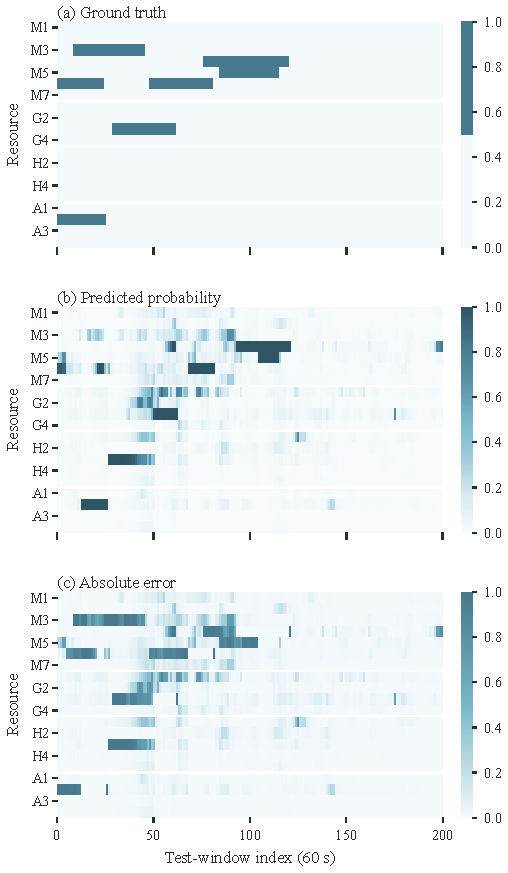
\includegraphics[width=0.90\textwidth,height=0.38\textheight,keepaspectratio]{figures/attention_heatmaps/fig08_prediction_heatmaps.pdf}
\caption{Future-event labels, predicted probabilities, and absolute errors for a mixed-disturbance episode (Start$\leq5$).}
\label{fig:attn-prediction}
\end{figure*}
